% Class Options (Optional)
%\PassOptionsToClass{sigconf, anonymous=true}{acmart} 
%\PassOptionsToClass{conference, nofonttune}{IEEETran}

% 1. Choose conference template "ieee", "acm", "lncs", or "elsevier"
% -----------------------------------------------------
\documentclass[conference, nofonttune]{template/ieee/IEEEtran}

% colors
\RequirePackage{xcolor}
\definecolor{col_link}{HTML}{0087BE}
\definecolor{col_prim}{HTML}{009999}
\definecolor{col_sec}{HTML}{00D7A0}  % bright: 00ffb9





% ----------------------------------------------------------------------
% Save \title, \author, \date before \maketitle
% \PassOptionsToPackage{pdfpagelabels, unicode=true}{hyperref}
\PassOptionsToPackage{pdfpagelabels}{hyperref}
\RequirePackage{hyperref}
\hypersetup{
    pdfcreator={LaTeX2e},
    pdfborder=0 0 0,
    breaklinks=true,
    bookmarksopen=true,
    bookmarksnumbered=true,
    linkcolor=col_link,
    urlcolor=col_link,
    citecolor=col_link,
    colorlinks=true
}


% Author Info
\gdef\theAuthorOneName{}
\gdef\theAuthorOneMail{}
\gdef\theAuthorOneOrg{}
\gdef\theAuthorOneCountry{}
\gdef\theAuthorOneORCID{}
\providecommand{\authorOneName}[1]{\gdef\theAuthorOneName{#1}}
\providecommand{\authorOneMail}[1]{\gdef\theAuthorOneMail{#1}}
\providecommand{\authorOneOrg}[1]{\gdef\theAuthorOneOrg{#1}}
\providecommand{\authorOneCountry}[1]{\gdef\theAuthorOneCountry{#1}}
\providecommand{\authorOneORCID}[1]{\gdef\theAuthorOneORCID{#1}}

\gdef\theAuthorTwoName{}
\gdef\theAuthorTwoMail{}
\gdef\theAuthorTwoOrg{}
\gdef\theAuthorTwoCountry{}
\gdef\theAuthorTwoORCID{}
\providecommand{\authorTwoName}[1]{\gdef\theAuthorTwoName{#1}}
\providecommand{\authorTwoMail}[1]{\gdef\theAuthorTwoMail{#1}}
\providecommand{\authorTwoOrg}[1]{\gdef\theAuthorTwoOrg{#1}}
\providecommand{\authorTwoCountry}[1]{\gdef\theAuthorTwoCountry{#1}}
\providecommand{\authorTwoORCID}[1]{\gdef\theAuthorTwoORCID{#1}}

\gdef\theAuthorThreeName{}
\gdef\theAuthorThreeMail{}
\gdef\theAuthorThreeOrg{}
\gdef\theAuthorThreeCountry{}
\gdef\theAuthorThreeORCID{}
\providecommand{\authorThreeName}[1]{\gdef\theAuthorThreeName{#1}}
\providecommand{\authorThreeMail}[1]{\gdef\theAuthorThreeMail{#1}}
\providecommand{\authorThreeOrg}[1]{\gdef\theAuthorThreeOrg{#1}}
\providecommand{\authorThreeCountry}[1]{\gdef\theAuthorThreeCountry{#1}}
\providecommand{\authorThreeORCID}[1]{\gdef\theAuthorThreeORCID{#1}}

\gdef\theAuthorFourName{}
\gdef\theAuthorFourMail{}
\gdef\theAuthorFourOrg{}
\gdef\theAuthorFourCountry{}
\gdef\theAuthorFourORCID{}
\providecommand{\authorFourName}[1]{\gdef\theAuthorFourName{#1}}
\providecommand{\authorFourMail}[1]{\gdef\theAuthorFourMail{#1}}
\providecommand{\authorFourOrg}[1]{\gdef\theAuthorFourOrg{#1}}
\providecommand{\authorFourCountry}[1]{\gdef\theAuthorFourCountry{#1}}
\providecommand{\authorFourORCID}[1]{\gdef\theAuthorFourORCID{#1}}

\gdef\theAuthorFiveName{}
\gdef\theAuthorFiveMail{}
\gdef\theAuthorFiveOrg{}
\gdef\theAuthorFiveCountry{}
\gdef\theAuthorFiveORCID{}
\providecommand{\authorFiveName}[1]{\gdef\theAuthorFiveName{#1}}
\providecommand{\authorFiveMail}[1]{\gdef\theAuthorFiveMail{#1}}
\providecommand{\authorFiveOrg}[1]{\gdef\theAuthorFiveOrg{#1}}
\providecommand{\authorFiveCountry}[1]{\gdef\theAuthorFiveCountry{#1}}
\providecommand{\authorFiveORCID}[1]{\gdef\theAuthorFiveORCID{#1}}


% Additional Info
\gdef\theDOI{}
\providecommand{\doi}[1]{\gdef\theDOI{#1}}

\gdef\theShortAuthorString{}
\providecommand{\shortAuthorString}[1]{\gdef\theShortAuthorString{#1}}

\gdef\thedoctype{}
\providecommand{\doctype}[1]{\gdef\thedoctype{#1}}


\gdef\thekeywords{}
\providecommand{\keywords}[1]{\gdef\thekeywords{#1}}



% Title
% \makeatletter
% \renewcommand{\title}[1]{%
%     \gdef\@title{#1}%
%     \gdef\thetitle{#1}
% }
% \makeatother


% set PDF properties
\makeatletter
\AddToHook{begindocument/end}{%

\@ifpackageloaded{hyperref}{%
  \hypersetup{%
    %bookmarks    = true,         % show bookmarks bar?
    %pdftoolbar   = true,         % show Acrobat’s toolbar?
    %pdfmenubar   = true,         % show Acrobat’s menu?
    % pdffitwindow = false,        % window fit to page when opened
    % pdfstartview = {FitH},       % fits the width of the page to the window
    pdftitle     = {\@title},  % title
    pdfauthor    = {\theShortAuthorString}, % author
    pdfsubject   = {\thedoctype},% subject of the document
    % pdfcreator   = {\theauthor}, % creator of the document
    pdfkeywords  = {\thekeywords}, 
    pdfnewwindow = true,         % links in new window
  }}{}%
}
\makeatother




\author{%
    \IEEEauthorblockN{\theAuthorOneName}%
    \IEEEauthorblockA{%
        \href{mailto:\theAuthorOneMail}{\theAuthorOneMail}\\%
        \theAuthorOneOrg, \theAuthorOneCountry
    }%
    \ifx\theAuthorTwoName\empty\relax\else
        \and
        \IEEEauthorblockN{\theAuthorTwoName}%
        \IEEEauthorblockA{%
            \href{mailto:\theAuthorTwoMail}{\theAuthorTwoMail}\\%
            \theAuthorTwoOrg, \theAuthorTwoCountry
        }%
    \fi
    \ifx\theAuthorThreeName\empty\relax\else
        \and
        \IEEEauthorblockN{\theAuthorThreeName}%
        \IEEEauthorblockA{%
            \href{mailto:\theAuthorThreeMail}{\theAuthorThreeMail}\\%
            \theAuthorThreeOrg, \theAuthorThreeCountry
        }%
    \fi
    \ifx\theAuthorFourName\empty\relax\else
        \and
        \IEEEauthorblockN{\theAuthorFourName}%
        \IEEEauthorblockA{%
            \href{mailto:\theAuthorFourMail}{\theAuthorFourMail}\\%
            \theAuthorFourOrg, \theAuthorFourCountry
        }%
    \fi
}%


\AddToHook{begindocument/end}{
    \markboth{}{}

    \bibliographystyle{template/ieee/IEEEtran}

    \maketitle

    \begin{abstract}%
        \ignorespaces% Short summary of the context, the problem, your approach and its experimental results.
% 2 sentences about scope and problem
Intelligent vehicles that autonomously plan, communicate, and perform intersection crossings will reduce accidents and delays compared to human drivers.
Previously proposed solutions require the use of additional expensive infrastructure, such as centralized Intersection Managers.

% 1-2 sentences main idea. Start new paragraph with "In this paper"
In this paper, we propose a decentralized intersection management that requires no additional infrastructure and can tolerate timing deviations due to unpredictable but detectable events, such as pedestrian movement or ambulances. 
Vehicles cooperate via direct VANET communication to agree on a schedule that specifies the groups and the order in which approaching vehicles will cross the intersection. 

% State your results in numbers
Our simulations show that CISCAV ensures safety and keeps the average delay in high traffic conditions at $\SI{32}{s}$, while conventional crossing policies, such as traffic lights, increase the delay up to $\SI{150}{s}$.%
    \end{abstract}
    \begin{IEEEkeywords}%
        \ignorespaces\thekeywords%
    \end{IEEEkeywords}

    %\IEEEpubid{\makebox[\columnwidth]{978-1-6654-3156-9/21/\$31.00~\copyright2021 IEEE \hfill} \hspace{\columnsep}\makebox[\columnwidth]{ }}

}



% 2. Add own packages here 
% -----------------------------------------------------
\RequirePackage{graphicx, microtype, booktabs, siunitx}
\RequirePackage[noabbrev,capitalize]{cleveref}  % adds \cref
\RequirePackage{flushend}      % auto-balance columns on last page
% % Squeeze Magic
% -----------------------------------------------------

% figures
\RequirePackage{caption}   % change figure captions

% title spacing
%\def\IEEEtitletopspace{-0.1cm}

% line distance (defautl 1.0)
\renewcommand{\baselinestretch}{0.98}  % or 0.94

% column separation (default 2pc)
% \setlength{\columnsep}{1.8pc}

\AtBeginDocument{
    % figures
    \captionsetup{font={small}}  % mod: \sf
    \captionsetup[figure]{belowskip=-7pt, aboveskip=6pt}
    \captionsetup[table]{belowskip=-10pt, aboveskip=6pt}
}

% -----------------------------------------------------



% 3. Specify Metadata
% -----------------------------------------------------

\title{An awesome paper template}

% comma-separated keywords (will be included in PDF metadata)
\keywords{Traffic Management, CPS, SUMO, IoT}

\doctype{Conference Paper}  % for PDF Metadata


% Author information. 
% First, specify a simple, short Author String that will be included in the header and PDF metadata. E.g. use "John Doe et. al." or "J. Doe, A. Smith, C. Hook"
\shortAuthorString{E. Regnath, J. Doe}


% Provide all author details
% Can use up to authorFiveXXX
\authorOneName{Emanuel Regnath}
\authorOneMail{emanuel.regnath@siemens.com}
\authorOneOrg{Siemens AG}
\authorOneCountry{Germany}
\authorOneORCID{0000-0002-0006-7761}

\authorTwoName{John Doe}
\authorTwoMail{john.doe@tum.de}
\authorTwoOrg{Technical University of Munich}
\authorTwoCountry{Germany}
\authorTwoORCID{}


% specify DOI for Camera Ready Version
%\doi{10.475/123_4}


% Begin of document. The template files use the hook "begindocument/end" to create the title area after this line and automatically insert the content of "content/0_abstract.tex" 
\begin{document}


% 4. Choose content sections to include
% -----------------------------------------------------
\section{Introduction}\label{sec:introduction}
% ---------------------------------------------
% goal: draw a picture of the context in which your work is embedded.

In the introduction, get the attention of the reader and draw a picture of the context in which your work is embedded. This should include:

\begin{itemize}
    \item Motivation: Describe the ultimate goal, the glory future that we want to reach.
    \item Problem Statement: Why is there currently a gap between us and our goal? What is the problem?
    \item Contributions: What will you do / have you done to narrow this gap?
\end{itemize}

For example, start with an interesting statistic:
Road intersections are not only a hot spot for accidents but also cause delays and congestions, especially in urban areas.
According to \cite{stau}, drivers in the US spend an additional 100 hours per year in their vehicles due to congestion and these delays have caused additional costs of 88 billion USD in 2019.





\subsection{Contributions}\label{sec:contributions}
Your contributions are of high interest to the reader. It is good practice to give them their own subsection to be easily spotted. In the best case this subsection is still visible on the first page.
Provide a short list of contributions that this paper provides and add forward references to the sections where they covered. 

For example: This paper addresses the scheduling problem for intersections and the required communication on an architectural level. We assume that once the vehicles have agreed on a schedule for crossing the intersection, they can execute a safe crossing autonomously.

In particular, we
\begin{itemize}
    \item propose a distributed intersection management scheme which uses consensus to agree on schedule groups (\cref{sec:approach}),%(\sectionref{sec:approach}).
    \item provide a \texttt{C++} implementation for the realistic simulation framework SUMO (\cref{sec:details}),
    \item discuss related approaches from literature and why they are over-optimistic (\cref{sec:related}),
    % (\sectionref{sec:sota})
    \item simulate and evaluate safety and delay (\cref{sec:evaluation}).
\end{itemize}



	% ===================================================
	\newcommand\circnum[1]{\textcolor{col_prim}{\textcircled{\raisebox{-0.9pt}{#1}}}}
	\begin{figure}[t]
	  \centering
	  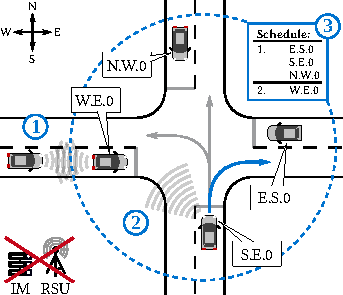
\includegraphics[width=\columnwidth]{res/img/idea}
	  \caption{Example Image of the main idea: Vehicles agree P2P on schedule groups using three communication phases: \circnum{1} Intra-Lane Exchange, \circnum{2} Inter-Lane Exchange, and \circnum{3} Schedule Group Consensus. No central Intersection Managers (IM) or Road-Side Units (RSU) are required.}
	  \label{fig:idea}
	\end{figure}
	% ===================================================


% \section{State of the Art}\label{sec:sota}
% ---------------------------------------------
% goal: Where is technology right now? How does it work? 
In this optional section, you can describe the established methods that already exist to solve the problem.
You should provide the information that is necessary for the reader to understand your approach. 
Other related research will be described later.


\section{Our XYZ Method}\label{sec:approach}
% ---------------------------------------------
% goal: Explain your concept to solve the problem. Intuition first, then all details



\section{Implementing XYZ}\label{sec:details}
% ---------------------------------------------
% goal: Explain your concept to solve the problem. Intuition first, then all details



\section{Related Work}\label{sec:related}
% ---------------------------------------------
% Goal: Which other ideas/approaches exist to solve the problem? How can they be categorized and how do they relate to your approach?

Related work is categorized in \cref{tab:sota}.

\begin{table*}[t]
    \def\noa{\textcolor{darkgray}{N/A}}
	\def\mps{\meter\per\second}
    \def\mpss{\meter\per\second\squared}
	\sisetup{per-mode = fraction}%
	\renewcommand{\arraystretch}{1.6}
	\centering
    \small
    \begin{tabular}{@{}llrlrrrll@{}} \toprule
    \multicolumn{2}{c}{Algorithm} & \multicolumn{2}{c}{Intersection} & \multicolumn{4}{c}{Vehicle} & Results\\  \cmidrule(rr){1-2}\cmidrule(lr){3-4}\cmidrule(lr){5-8}\cmidrule(ll){9-9}
    \textbf{Name}  & \textbf{Simulation} & \textbf{S/L} & \textbf{Legs/Near} & \textbf{L} $[\si{m}]$ & \textbf{V} $\left[\si{\meter\per\second}\right]$ & \textbf{Acc.} $\left[\si{\meter\per\second\squared}\right]$ & \textbf{L-S-R} [\%] & \textbf{Avg. Delay}\\ \midrule
		AIM08 \cite{im_aim08}    & Custom            & +1 & \SI{125}{m}/--         & \noa & \num{25.0} & \noa & 0-100-0 & \SI{0.2}{s}@\SI{0.5}{v/s/ln}\\
		Prio14 \cite{im_priority14}  & SUMO/\SI{10}{min} & +3 & \SI{290}{m}/\SI{50}{m} & \noa & \num{12.0} & $-4\,..\,2$ & 20-70-10 & \SI{15}{s}@\SI{0.5}{v/s/rd}\\ 
		Delay17 \cite{im_delay17} & SUMO & +1 & \SI{50}{m}/\SI{50}{m} & \noa & \noa & \noa & 20-70-10 & $\SI{35}{s}@\SI{0.5}{v/s/rd}$\\ 
        CISCAV (ours)  & SUMO / \SI{3600}{s} & +1  & \SI{200}{m}/\SI{100}{m}     & $4.3$ & \num{13.9} & $-7.5\,..\,2.9$ & 33-33-33 & \SI{32}{s}@\SI{0.5}{v/s/rd} \\
        \bottomrule
	\end{tabular}
	\caption{Example table to show related work. \textbf{S/L} indicates the shape of the intersection ($\vdash$, $+$, $+\hspace*{-0.8em}\times$) and the number of \emph{incoming} lanes for each direction. \textbf{Legs/Near} is the length of the intersection roads per leg and the distance from the center at which vehicles start broadcasting messages. \textbf{L, V, Acc.} states the vehicle \textit{L}ength; max. \textit{V}elocity; and maximum deceleration (negative) and \textit{Acc}eleration considered. \textbf{L-S-R} are the probabilities for a vehicle to turn left (L), go straight (S), or turn right (R) in percent. Each related approach did not mention at least one of these parameters (\noa).}
	\label{tab:sota}
\end{table*}		


\section{Evaluation}\label{sec:evaluation}
% ---------------------------------------------
% Goal: Demonstrate how well your approach works and compare its performance to related work.

\subsection{Metrics}\label{sec:metrics}
% Clearly define what and how you measure

We evaluate our approach based on three important metrics: 
\begin{enumerate}
	\item \textbf{Delay} is the \emph{additional time} for a vehicle to completely cross an intersection compared to a crossing where the vehicle has priority from the beginning and can cross without any interactions with other vehicles.
	\item \textbf{Stop Time} is the total duration a vehicle has a velocity lower than \SI{0.1}{m/s}.
	\item \textbf{Communication Overhead} the average number of bytes a vehicle needs to send.
\end{enumerate}



\subsection{Experimental Setup}\label{sec:setup}
% Describe all the steps required to reproduce your results

In SUMO \cite{sumo}, we have created random traffic flows for a 4-leg intersection. We randomly spawn vehicles at the beginning of the roads (\SI{200}{m} from the center) with a given probability that is equal for all directions. For example, \SI{0.5}{v/s/rd} means that on average 0.5 vehicles will be spawned per second at each road. Spawned vehicles have equal probabilities ($33.\overline{3}$\%) to go in the following directions: left, straight, or right. We spawn vehicles over a period of \SI{3600}{s} and run the simulation until every vehicle has crossed the intersection. 
We have performed this experiment for varying spawn probabilities over 3 crossing policies: Traffic light, priority road, and CISCAV. 
% \section{Discussion}\label{sec:discuss}
% ---------------------------------------------
% Goal: Explain where, why, and to which extend you have or have not improved over related work. What does this mean for your initial problem question?



\section{Conclusion}\label{sec:conclusion}
% ---------------------------------------------
% Goal: Summarize main points; formulate key message. Remind the readers what they have read and why it was significant. Don’t give new explanations, just the facts. Repeat the most important result (number!) and what it means for the problem.



	


% 5. Compile!

% references are added at the end
\vfill
\bibliography{res/bib/references}
\vspace{-0.3em}

% that's all folks
\end{document}